\chapter{Literature-review} \label{Chapter: 2}
%% 1 -- 10 ohm Neutral grounding resistance in 30kV western Libyan network and effects
\ifdraft{
The history of the transformer may be found in the early 1800's where the discovery of the property of induction and the invention of the induction coil. It was between 1880 to 1882 that Sebastian Ziani de Ferranti with William Thomas designed one of the earliest AC power systems. Lucien Gaulard and John Dixon Gibbs built the first step down transformer in 1882 with an open iron core that was first shown in exhibition in Italy 1884 but was not efficient enough to make and work with.  In 1884, Ottó Bláthy, Károly Zipernowsky and Miksa Derí came up with the first closed built transformer with toroidal shape. It was not until William Stanley who went to the exhibition in Italy and saw the open iron core step down transformer. After the exhibition his boss George Westinghouse bought the patent to the Gaulard and Gibbs transformer design.  George W. and William S. created a transformer that was more practical in production than the Gaulard and Gibbs.  They changes the shape from toroidal shape that was hard to wind the wire around to a square shape that was much easier to work with. Mikhail Dolivo-Dobrovolsky a Russian born engineer who was working at AEG in Germany developed the first three-phase transformer that was used in the first powerful AC system\footnote{\url{http://www.edisontechcenter.org/Transformers.html}}.


%\section{10 ohm Neutral grounding resistance in 30kV western Libyan network and effects}
%In a 30kV (kilo Volt) network that is limited to the single line to ground fault current which is by connecting a 10 ohm neutral-grounding resistance that could lead to a possible reduced danger of too high potential gradients.    
%hallo 
}{}
\newpage
\section{The Working of a Transformer}
\ifdraft{
Some characteristic of a transformer is that there are no moving parts, efficiency is very high and the frequency between windings are unchanged. \cite{Salam_2016}  As from figure \ref{Fig: Ideal transformer with two winding on a single core} it shows a single phase transformer.  The core is made of magnetic materials that enable the magnetic flux $\phi$ when current goes through winding N$_p$.  The flux created by N$_p$ goes through the core and connects with N$_s$.  In a ideal transformer there is no loss in the transformer and is used for easier calculation, in real transformer there is energy loss in every step of the process but that is determined by the material used. The companies that make transformers have different ways of making the transformer and in many instances they are costume made for specific porpoise. From equation \ref{Math: Voltage, Current and Turns ratio} it shows there is a correlation between the ratio of primary and secondary windings and the input and output of voltage and current. Since the transformer is a critical equipment for the use of distribution of electricity then a good protection system is needed to keep the transformer active.  The time the transformer is connected it needs to stay on at all time unless it is taken out of service for some reason.  
The connection between windings on a transformer can be be wye (Y) or delta ($\Delta$).  There are 4 possible different ways of connection and are 
\begin{itemize}
\item  Y-Y (wye-wye)
\begin{figure}[h!]
\center
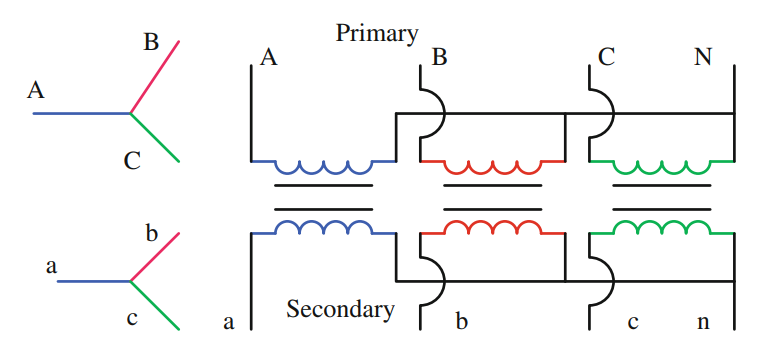
\includegraphics[scale=0.45]{graphics/Y_Y_Connection.PNG}
\caption{Y-Y connection diagram}
\end{figure}
\newpage
\item Y-$\Delta$ (wye-delta)
\begin{figure}[h!]
\center
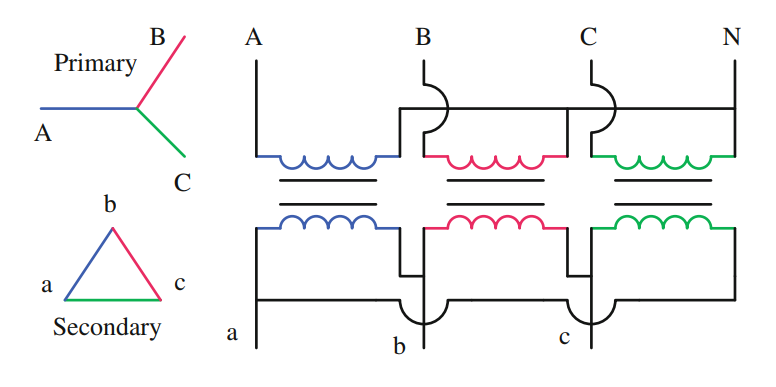
\includegraphics[scale=0.45]{graphics/Y_D_Connection.PNG}
\caption{Y-$\Delta$ connection diagram}
\end{figure}
\item $\Delta$- Y (delta-wye)
\begin{figure}[h!]
\center
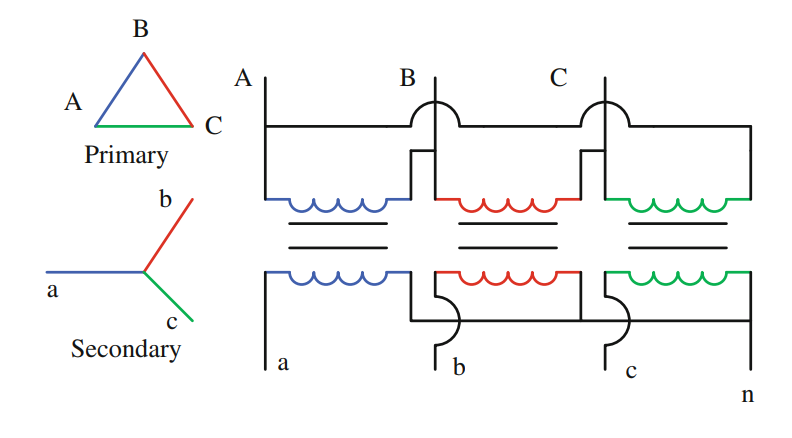
\includegraphics[scale=0.45]{graphics/D_Y_Connection.PNG}
\caption{$\Delta$-Y connection diagram}
\end{figure}
\item $\Delta$-$\Delta$ (delta - delta)
\begin{figure}[h!]
\center
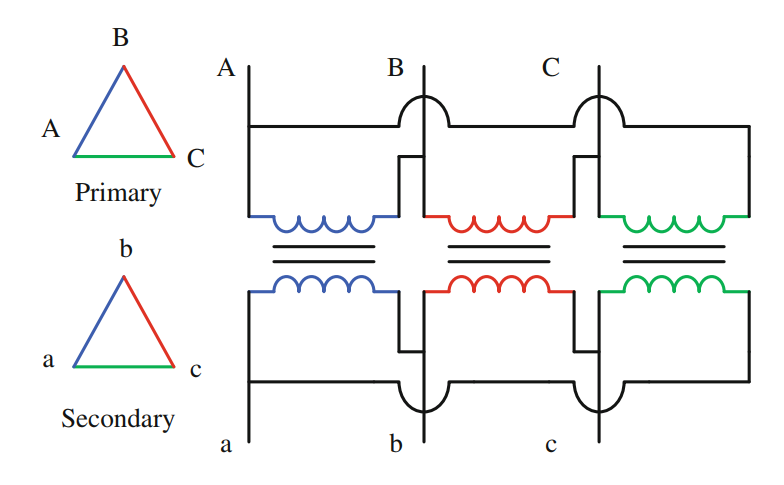
\includegraphics[scale=0.45]{graphics/D_D_Connection.PNG}
\caption{$\Delta$-$\Delta$ connection diagram}
\end{figure}
\end{itemize}  
The mainly used connection for a step down transformer is the Y-$\Delta$ (wye-delta) and for a step up is $\Delta$- Y (delta-wye)\cite{Salam_2016}[p. 88].
}{}

\section{Transformer Protection}
\ifdraft{
Since the transformer is very critical and expensive, the protection system needs to keep the transformer safe for operational use and here is listed some protective functions \cite{Constantin_2012}
\begin{itemize}\label{List: Transformer Protection systemms}
\itemsep0em 
\item Transformer Differential (87T)
\item Restricted earth fault or ground differential protection (87GN)
\item Instantaneous and inverse time Overcurrent (50$/$51)
\item Ground instantaneous and inverse time Overcurrent (50G/51G)
\item Current Unbalance/Negative Sequence (46)
\item Over-excitation (24)
\item Under-voltage (27)
\item Over-voltage (59)
\item Under-frequncy (81U)
\item Thermal Protection (49)
\item Breaker failure (50BF)
\end{itemize}
where the parenthesis numbers represent the ANSI device function.

\subsection{Transformer Differential (87T)}
Differential protection \cite{Trans_Diff87T} uses sensors on the primary and secondary connections that compares the two currents of the same phase.  If the currents equal each other than it is normal operation.  If the currents do not equal each other then the transformer is not in working correctly. The currents have amplitude difference between the primary and secondary because of phase difference because coupling in the transformer and ratio of current transformation.
The current matching of the primary winding is the same way of all vector shifts of the transformer.
\begin{equation}
\begin{split}
I_{1m} = \dfrac{I_{1p}}{ln(1)}- \dfrac{I_{1p}+I_{2p}+I_{3p}}{3ln(1)}\\
I_{2m} = \dfrac{I_{2p}}{ln(1)}- \dfrac{I_{1p}+I_{2p}+I_{3p}}{3ln(1)}\\
I_{3m} = \dfrac{I_{3p}}{ln(1)}- \dfrac{I_{1p}+I_{2p}+I_{3p}}{3ln(1)}\\
\end{split}
\end{equation} 
Where $I_{1m},I_{2m},I_{3m}$ is the matching value. $I_{1p},I_{2p},I_{3p}$ is the current value from the primary windings. See figure \ref{Fig: Vector shifts of transformer} for matching value for the second winding respective from vector shift. \cite{Trans_Diff87T}[p. 6]
\newpage
\begin{figure}[h!]
\center
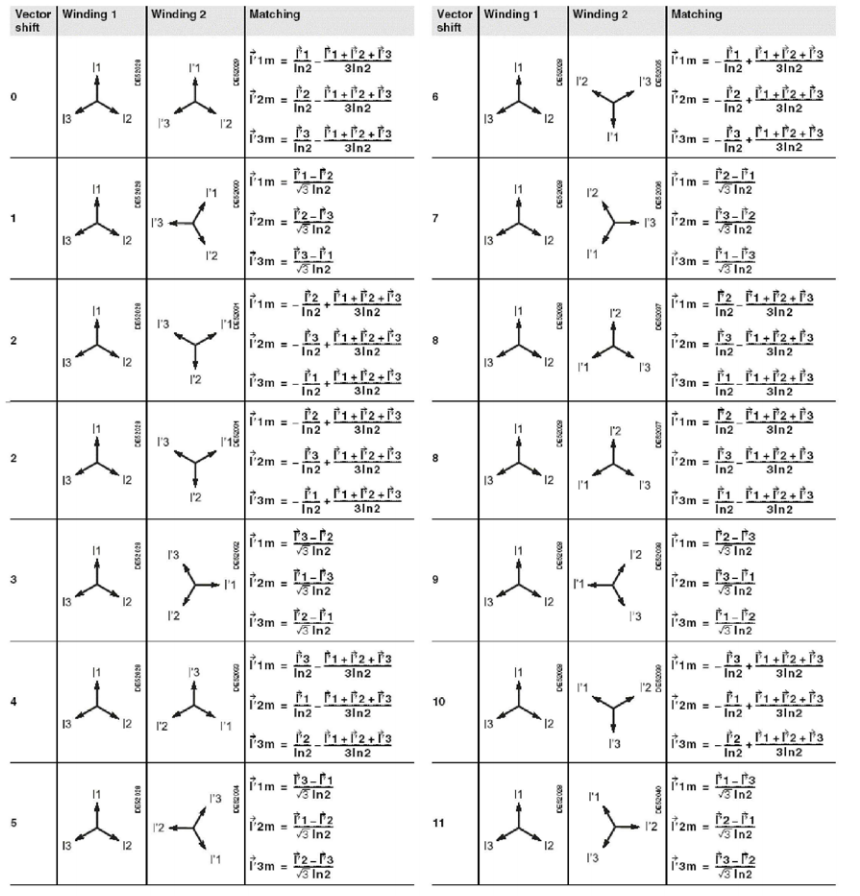
\includegraphics[scale=0.8]{graphics/Vector_Shift.png}
\caption{Vector Shifts of the Transformer with 123 type phase-rotation sequences}
\label{Fig: Vector shifts of transformer}
\end{figure}
}{}

\subsection{Restricted earth fault or ground differential protection (87GN)}
\ifdraft{The 87GN ground protection is sensitive enough to detect internal ground faults. It uses low-resistance grounded  .Fig \ref{Fig: Ground Differential Protection} shows the set up and is able to detect ground faults without false tripping on external faults \cite{Pillai_2004} \cite{Ramon_Ferran}.
\newpage
\begin{figure}[h!]
\center
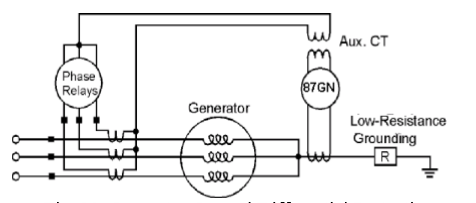
\includegraphics[scale=0.8]{graphics/Ground_Differential_Protection.PNG}
\caption{Ground Differential Protection}
\label{Fig: Ground Differential Protection}
\end{figure} 
}

\subsection{Ground instantaneous and inverse time Overcurrent (50G/51G)}
\ifdraft{
Figure \ref{Fig: Ground time and overcurrent protection} shows the set up for the 50G and 51G where they work together for using 50G overcurrent relays that are positioned on each feeder and using 51G inverse time overcurrent on the grounded neutral sources.  51G provideds protection against exernal faults if the 50G has not isolated the fault.  \cite{Pillai_2004} \cite{Ramon_Ferran}.
\begin{figure}[h!]
\center
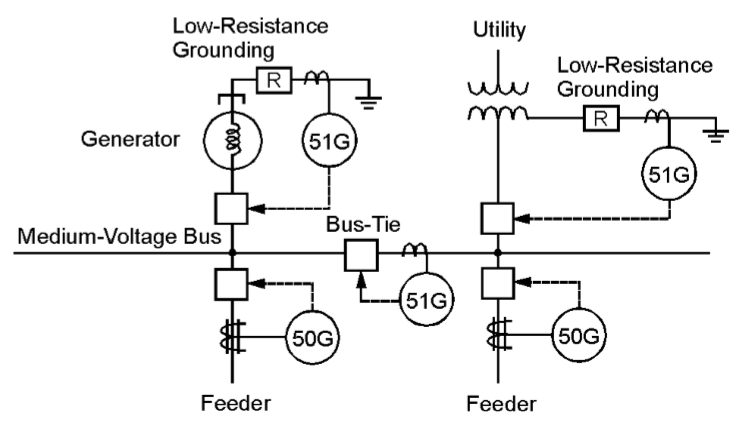
\includegraphics[scale=0.5]{graphics/Ground_Instantaneous_and_inverse_time_Overcurrent.PNG}
\caption{Ground time and overcurrent protection}
\label{Fig: Ground time and overcurrent protection}
\end{figure}

\subsection{Thermal Protection (49)}
When the transformer is turn on the electricity flows through it, the loss of power in the transformer is turned to heat.  

}

%\subsection{M-C system}

\subsection{Transformer fault}
\ifdraft{
The potential faults that happens in a transformer\\
Winding failure:
\begin{itemize}
\item turn-to-turn insulation failure
\item moisture
\item deterioration
\item phase-to-phase and ground faults
\item external faults (producing insulation failure
\end{itemize}
Tap changer failure:
\begin{itemize}
\item mechanical
\item electrical
\item short circuit
\item oil leak
\item overheating
\end{itemize}
Bushing failure:
\begin{itemize}
\item ageing, contamination and cracking
\item flash-over due to animals
\item moisture
\item low oil
\end{itemize}
Core failure:
\begin{itemize}
\item core insulation failure
\item ground strap burned away
\item loose clamps, bolts, wedges
\end{itemize}
Miscellaneous failure
\begin{itemize}
\item Bushing CT failure
\item metal particles in oil
\item damage in shipment
\item external faults
\item poor tank weld
\item over voltages
\item overloads
\end{itemize}
}

\subsection{Detection of transformer internal faults}
\ifdraft {
Phase-to-phase
\begin{itemize}
\item transformer differential protection
\item Buchholz relay
\item overpressure device
\item under-impedance/distance device
\item HV fuses
\end{itemize}
Ground-fault, low impedance
\begin{itemize}
\item restricted ground-fault protection
\item transformer differential protection
\item Buchholz relay
\item under-impedance/distance device
\item HV fuses
\end{itemize}
Ground-fault, high impedance grounding
\begin{itemize}
\item restricted ground-fault protection
\item sensitive ground-fault current protection
\item neutral (residual) over-voltage protection
\item Buchholz gas alarm
\end{itemize}
Turn-to-turn fault
\begin{itemize}
\item Buchholz alarm
\item transformer differential protection
\end{itemize}
HV to LV winding flash-over
\begin{itemize}
\item transformer differential protection
\item Buchholz relay
\item overpressure device (sudden pressure relay)
\end{itemize}

}

%%% Local Variables: 
%%% mode: latex
%%% TeX-master: "MSC-Kristján-2018"
%%% End: 
